% Sokoban AI - sprawozdanie z benchmarkiem z 12.11.2026.
% Kompilator Overleaf: pdfLaTeX.
\documentclass[a4paper,11pt]{article}

\ifdefined\XeTeXversion
  \usepackage{fontspec}
\else
  \usepackage[T1]{fontenc}
  \usepackage[utf8]{inputenc}
  \usepackage{lmodern}
\fi
\usepackage[polish]{babel}
\usepackage{microtype}
\usepackage{geometry}
\geometry{margin=2.25cm}
\usepackage{amsmath,amssymb}
\usepackage{booktabs,tabularx,array}
\usepackage{graphicx}
\usepackage{float}
\usepackage{tikz}
\usetikzlibrary{arrows.meta,positioning}
\usepackage{enumitem}
\usepackage{xcolor}
\usepackage{hyperref}
\hypersetup{colorlinks=true,linkcolor=blue!55!black,urlcolor=blue!55!black,citecolor=blue!55!black}
\usepackage{fancyhdr}
\usepackage{lastpage}
\setlength{\parindent}{0pt}
\setlength{\parskip}{0.45em}
\setlist[itemize]{nosep,leftmargin=*}
\setlist[enumerate]{nosep,leftmargin=*}
\renewcommand{\arraystretch}{1.17}
\setlength{\headheight}{14pt}
\pagestyle{fancy}
\fancyhf{}
\cfoot{\thepage/\pageref{LastPage}}
% Wygenerowano przez aggregate_benchmark.py na podstawie benchmark_raw.csv.
\newcommand{\HeuristicSummaryRows}{%
STEPS & $h_1$ & 36/36 & 217\,690 & 248\,401 & 34,08 \\
STEPS & $h_2$ & 36/36 & 217\,690 & 248\,401 & 35,04 \\
STEPS & $h_3$ & 36/36 & 197\,302 & 225\,503 & 32,37 \\
ENERGY & $h_1$ & 36/36 & 280\,371 & 303\,277 & 43,92 \\
ENERGY & $h_2$ & 35/36 & 237\,184 & 259\,402 & 38,60 \\
ENERGY & $h_3$ & 36/36 & 181\,903 & 188\,197 & 29,26 \\
}
\newcommand{\LastLevelRows}{%
STEPS & $h_1$ & 78\,812 & 90\,751 & 13,28 \\
STEPS & $h_2$ & 78\,812 & 90\,751 & 13,60 \\
STEPS & $h_3$ & 64\,912 & 74\,834 & 11,62 \\
ENERGY & $h_1$ & 98\,730 & 105\,663 & 16,86 \\
ENERGY & $h_2$ & 97\,187 & 104\,120 & 16,88 \\
ENERGY & $h_3$ & 59\,039 & 59\,821 & 10,07 \\
}
\newcommand{\EnergyTradeoffRows}{%
6. Ciężarowiec & 34/36 & 6\,481,96 & 6\,364,24 & 117,72 & 1,82 \\
10. Lodowe beczki & 31/31 & 4\,167,03 & 4\,080,71 & 86,33 & 2,07 \\
12. Wielki magazyn & 52/55 & 7\,401,58 & 7\,340,57 & 61,01 & 0,82 \\
}


\begin{document}

\begin{center}
    {\Large\bfseries Sokoban AI -- planowanie ruchów\\z uwzględnieniem ograniczeń fizycznych\par}
    \vspace{0.55em}
    {\large Sprawozdanie z projektu nr 5}\par
    \vspace{0.45em}
    {\normalsize Sztuczna inteligencja w grach i rozszerzonej rzeczywistości}\par
    \vspace{0.65em}
    {\normalsize \textbf{Autorzy:} Alicja Borek, Radosław Firlej, Mariusz Wątroba}\par
\end{center}

\textbf{Streszczenie.} Opracowano grę Sokoban w silniku Godot z algorytmem A* i dyskretnym modelem fizycznym współdzielonym z rozgrywką. Uwzględniono masy obiektów, przyczepność robota, tarcie, poślizg, toczenie beczek, drzwi sterowane płytami naciskowymi i jednokierunkowe uskoki. Na 12 planszach porównano trzy heurystyki w dwóch trybach kosztu. W 216 próbach uzyskano 215 poprawnych planów i jedno przekroczenie limitu czasu. W ENERGY heurystyka Terrain-Aware zmniejszyła liczbę rozwinięć w całej kampanii o 35,1\% względem Manhattan przy tym samym koszcie planów.

\section{Cel projektu i założenia}
Zadaniem agenta jest umieszczenie skrzyń lub beczek na wszystkich polach docelowych bez naruszania reguł gry; część poziomów zawiera także nadmiarowe obiekty potrzebne do aktywowania płyt. Stan może stać się nierozwiązywalny wskutek zablokowania skrzyni przez przeszkody lub ograniczenia fizyczne. Dlatego celem nie jest wyłącznie znalezienie dowolnej ścieżki, ale również analiza kosztu rozwiązania i sytuacji bez wyjścia (\emph{deadlocków}).

Projekt rozszerzono w dwóch obszarach: (1) model fizyczny, który wpływa na dostępne ruchy i ich koszt, oraz (2) interaktywna gra 2D wykonana w Godot Engine 4, umożliwiająca ręczną rozgrywkę i prezentację działania AI.

\textbf{Zakres oceny:} odsetek rozwiązanych poziomów, długość planu, zużycie energii, liczba rozwiniętych/odkrytych stanów oraz czas obliczeń. Wnioski opieramy na powtarzalnych testach tych samych plansz.

\section{Architektura rozwiązania}
System rozdziela warstwę wizualną, reprezentację stanu i algorytm od fizycznych reguł ruchu. Dane poziomu (\texttt{LevelData}) zawierają kafelki, cele, typy i masy obiektów, siłę robota oraz parametry płyt naciskowych. \texttt{BoardState} opisuje pozycję robota i pozycje, masy oraz rodzaje przesuwanych obiektów. Przejścia są obliczane przez \texttt{PhysicalModel.move()}, wykorzystywany zarówno przez grę, jak i solver.

\begin{figure}[H]
\centering
\begin{tikzpicture}[
  box/.style={draw=blue!45!black,rounded corners=3pt,fill=blue!3,align=center,minimum height=0.85cm,text width=3.8cm,font=\small},
  line/.style={-{Latex[length=2mm]},thick,draw=black!65},
  node distance=1.0cm and 1.65cm
]
\node[box] (ui) {Godot 4\\\texttt{game.gd}, HUD, animacje};
\node[box,right=of ui] (state) {Stan gry i poziom\\\texttt{BoardState}, \texttt{LevelData}};
\node[box,right=of state] (solver) {Planowanie A*\\heurystyki, statystyki};
\node[box,below=1.35cm of state] (physics) {Wspólny model fizyczny\\\texttt{PhysicalModel.move()}};
\draw[line] (ui) -- node[above,font=\scriptsize]{sterowanie} (state);
\draw[line] (state) -- node[above,font=\scriptsize]{stan i mapa} (solver);
\draw[line] (solver.south) |- (physics.east);
\draw[line] (state.south) -- (physics.north);
\draw[line] (physics.west) -| (ui.south);
\end{tikzpicture}
\caption{Uproszczony schemat logiczny architektury. Solver i rozgrywka korzystają z tych samych reguł przejścia.}
\label{fig:architecture}
\end{figure}

W HUD można wybrać poziom kampanii, kryterium kosztu (STEPS/ENERGY) i jedną z trzech heurystyk, ustawić maksymalną siłę robota, uruchomić AI i prześledzić wizualizowany plan. Przycisk zatrzymania przerywa odtwarzanie kolejnych ruchów. Kampania obejmuje 12 poziomów z zapisem postępów do pliku \texttt{user://progress.cfg}.

\section{Model fizyczny i reprezentacja stanu}
\subsection{Parametry i dopuszczalność ruchu}
Model jest dyskretny: $d=1\,\mathrm{m}$ oznacza długość pola, $g=9{,}81\,\mathrm{m/s^2}$ przyspieszenie ziemskie, a masa robota wynosi $m_r=40\,\mathrm{kg}$. Rzeczywista siła, którą robot może przekazać pchanemu obiektowi, zależy nie tylko od silnika, lecz również od przyczepności $\gamma$ podłoża pod robotem:
\begin{equation}
  F_{\mathrm{eff}}=\min\!\left(F_{\max},\ \gamma m_r g\right).
  \label{eq:force}
\end{equation}
Dla skrzyni o masie $m_i$ wymagana siła ruszenia jest równa $F_{\mathrm{start}}=m_i g\mu_s$. Dla beczki opór toczny $\rho$ zastępuje współczynnik tarcia: $F_{\mathrm{start}}=2m_i g\rho$. Pchnięcie jest dozwolone, gdy $F_{\mathrm{eff}}\geq F_{\mathrm{start}}$ oraz pole docelowe jest dostępne.
\begin{table}[H]
\centering\small
\caption{Podstawowe parametry terenu używane w modelu fizycznym.}
\label{tab:terrain}
\begin{tabular}{@{}lcccc@{}}
\toprule
Podłoże & $\mu_s$ & $\mu_k$ & $\gamma$ & $\rho$ \\
\midrule
Drewno i cel & 0,35 & 0,25 & 0,90 & 0,015 \\
Lód & 0,05 & 0,03 & 0,10 & 0,010 \\
Piasek & 0,75 & 0,65 & 0,60 & 0,300 \\
\bottomrule
\end{tabular}
\end{table}
Przyczepność ogranicza siłę na śliskim podłożu, nawet jeśli $F_{\max}$ jest wysokie. Poziomy zawierają ponadto płyty naciskowe otwierające drzwi po ich odpowiednim obciążeniu oraz uskoki, na które można wjechać tylko w kierunku strzałki. Warunki te są sprawdzane w \texttt{PhysicalModel.move()} zarówno podczas gry, jak i podczas planowania.

\subsection{Energia i poślizg}
Koszt zwykłego kroku robota wyraża $W_r=m_rg\mu_k d$, gdzie współczynnik $\mu_k$ pochodzi z pola startowego robota. Pchnięcie dodaje pracę przeciw oporowi kinetycznemu obiektu (dla skrzyń $m_i g\mu_kd$, dla beczek $m_i g\rho d$). Jeżeli obiekt wjeżdża na śliskie podłoże, otrzymuje dodatkową energię kinetyczną
\begin{equation}
 E_{\mathrm{start}}=\max(0,F_{\mathrm{eff}}-F_{\mathrm{start}})\,d.
\end{equation}
Na kolejnych polach poślizgu energia maleje o $m_i g(\mu_{k,i}+\mu_{k,i+1})d/2$ (dla beczek zamiast $\mu_k$ stosowany jest $\rho$). Ciało zatrzymuje się po wyczerpaniu energii, przed przeszkodą lub po wjechaniu na pole o większym oporze. Robot także może prześlizgnąć się przez kilka pól lodu, aż odzyska przyczepność lub napotka przeszkodę. Całkowity koszt akcji zwraca model fizyczny; interfejs nie oblicza go ponownie.

W modelu nie symuluje się ciągłego czasu, prędkości ani zderzeń: przesunięcia i zatrzymania są rozpatrywane w pozycjach kafelkowych. Funkcja przejścia zwraca całą trasę obiektu lub robota, dzięki czemu animacje i walidacja planów odpowiadają logice solvera.

\section{Algorytm A*, heurystyki i wykrywanie blokad}
\subsection{Przeszukiwanie stanów}
A* wybiera stan o najmniejszej wartości
\begin{equation}
  f(n)=g(n)+h(n),
\end{equation}
gdzie $g(n)$ to koszt dotychczasowej ścieżki, a $h(n)$ oznacza oszacowanie kosztu pozostałego do celu. Rozpatrywane są cztery kierunki ruchu, a ruch może powodować wielopolowy poślizg. Stan opisuje pozycję robota oraz pozycje, masy i rodzaje obiektów; klucz stanu nie zależy od ich kolejności w tablicy. Wyszukiwanie przechowuje najlepszy koszt dla odwiedzonych stanów i rekonstruuje akcje z relacji poprzedników.

Dwa tryby kosztu to \texttt{STEPS} (każda akcja kosztuje 1) i \texttt{ENERGY} (koszt w dżulach zwracany przez model). Każda heurystyka zwraca oszacowanie w jednostkach wybranego trybu. Kolejka priorytetowa jest kopcem binarnym. Po znalezieniu tańszej drogi do znanego stanu solver może rozwinąć go ponownie.

\subsection{Heurystyki}
\begin{table}[H]
\centering\small
\caption{Heurystyki zastosowane w algorytmie A*.}
\label{tab:heuristics}
\begin{tabularx}{\linewidth}{@{}>{\raggedright\arraybackslash}p{2.5cm}X@{}}
\toprule
Wariant & Sposób szacowania kosztu \\
\midrule
$h_1$ Manhattan & Odległość od najbliższego celu podzielona przez maksymalną długość poślizgu i zaokrąglona w górę. W ENERGY każde tak oszacowane pchnięcie kosztuje co najmniej minimalną pracę robota. \\
$h_2$ masa i tarcie & Granicę długości pchnięcia wyznacza osobno dla skrzyni i beczki. W ENERGY dolicza minimalną pracę potrzebną do przesunięcia danego obiektu, proporcjonalną do jego masy i najniższego oporu na planszy. \\
$h_3$ Terrain-Aware & Wyznacza odległość do najbliższego celu po odwróconych krawędziach uproszczonego grafu pchnięć, metodą Dijkstry startującą jednocześnie z wszystkich celów. Graf zależy od rodzaju i masy obiektu. \\
\bottomrule
\end{tabularx}
\end{table}
Graf $h_3$ wykorzystuje \texttt{PhysicalModel.push\_box()}, dzięki czemu uwzględnia ściany, kierunek uskoków, siłę robota, przyczepność i poślizg. Przyjmuje otwarte drzwi oraz dostęp robota do każdego pola, z którego może rozpocząć pchnięcie. Dopuszcza zatrzymanie na dowolnym polu fizycznie możliwej trajektorii, bo w rzeczywistej grze przeszkoda może skrócić poślizg. Krawędź kosztuje jeden ruch albo energię danego pchnięcia. Jeśli za mało obiektów może dotrzeć do celu w uproszczonym grafie, używa skończonego oszacowania $h_2$.

Wszystkie warianty sumują tyle najmniejszych oszacowań, ile jest celów. Dopuszczenie wspólnego celu dla kilku obiektów, pominięcie kosztu dojścia robota i uproszczenia przejść zapewniają dolne oszacowanie kosztu. Na małych planszach z lodem, beczką zatrzymywaną przez inną skrzynię i drzwiami otwieranymi płytą testy potwierdziły zgodność kosztu $h_2$ i $h_3$ z Dijkstrą ($h\equiv0$) w obu trybach.

\subsection{Detekcja deadlocków}
Solver wykrywa \emph{statyczne narożniki}: pola poza celami, mające ściany po dwóch prostopadłych stronach. Obiektu wepchniętego do takiego narożnika nie da się już wypchnąć. Algorytm odrzuca stan, gdy liczba obiektów niezablokowanych spada poniżej liczby celów. Nadmiarowe obiekty mogą pozostać poza celami, np. jako obciążniki płyt.

\section{Środowisko gry w Godot}
Gra wykorzystuje Godot Engine 4.7.2 (GDScript), sterowanie ręczne, HUD, animacje ruchu i poślizgu, wybór kryterium kosztu, regulację $F_{\max}$ oraz podgląd planu AI. Plansze są rysowane programowo, a ruchy odtwarzane przez model fizyczny identyczny jak podczas planowania. Kampania ma 12 kolejno odblokowywanych poziomów, a po ich ukończeniu zapisuje najlepszy wynik i postępy gracza. Nowe mechaniki obejmują beczki, płyty i drzwi oraz jednokierunkowe uskoki.

Wyszukiwanie A* jest synchroniczne i może na wymagających poziomach przejściowo blokować okno. Wyniki planowania obejmują status, liczbę ruchów, energię, czas oraz liczbę rozwiniętych i odkrytych stanów.

\section{Metodyka eksperymentów}
\subsection{Zestaw danych i warunki odtwarzania}
Badano 12 poziomów kampanii zapisanych w JSON, od \emph{Pierwszych kroków} do \emph{Wielkiego magazynu}. Plansze zespołu wprowadzają kolejno m.in. poślizg, piasek, ciężkie skrzynie, beczki, uskoki i płyty naciskowe. Każdą kombinację planszy, heurystyki i trybu kosztu uruchomiono trzy razy od tego samego stanu początkowego: $12\cdot3\cdot2\cdot3=216$ prób. Wyszukiwania wykonywano kolejno w jednym procesie Godota bez okna. Między powtórzeniami rotowano kolejność heurystyk i zmieniano kolejność trybów kosztu.

Użyto Godot 4.7.2 stable na Windows (kompilacja 26200), procesorze Intel Core i5-12500H i ok.\ 15,7 GiB pamięci fizycznej. Każda próba korzystała z siły robota zapisanej w JSON (300 N na wszystkich planszach) i limitów gry: 100\,000 rozwinięć oraz 30\,000 ms wyszukiwania. Wykrywanie blokad narożnych było włączone w każdej próbie.

Pomiar obejmował utworzenie heurystyki i pracę solvera, w tym budowę grafu $h_3$. Wczytanie poziomu i odtwarzanie planu odbywały się poza pomiarem. Dla każdej konfiguracji raportowano medianę czasu udanych prób oraz przedział min--max w CSV. Liczba odkrytych stanów oznacza liczbę różnych kluczy stanu w mapie najlepszych kosztów. Licznik rozwinięć uwzględnia także powtórne rozwinięcia tego samego stanu.

\subsection{Porównania i weryfikacja}
\begin{itemize}
\item \textbf{Porównanie heurystyk.} Na każdej planszy i dla każdego trybu porównano status, koszt optymalizowany, liczbę rozwiniętych i odkrytych stanów oraz czas dla $h_1$, $h_2$ i $h_3$.
\item \textbf{Porównanie kryteriów kosztu.} Dla planów wyznaczonych z $h_1$ porównano liczbę ruchów i rzeczywiste zużycie energii w STEPS i ENERGY. Porównanie pokazuje wpływ wyboru funkcji celu przy stałej heurystyce.
\end{itemize}

Każdy znaleziony plan ponownie wykonano przez \texttt{PhysicalModel.move()} od stanu początkowego. Sprawdzono legalność wszystkich akcji, zajęcie wszystkich celów, długość planu, sumaryczną energię i zgodność z optymalizowanym kosztem. Status \texttt{time\_limit} lub \texttt{state\_limit} pozostawia rozwiązywalność planszy nieustaloną.

\clearpage
\section{Wyniki i interpretacja}
\subsection{Porównanie heurystyk}
Każda heurystyka rozwiązała wszystkie 12 poziomów w obu trybach przynajmniej raz. Odtworzenie potwierdziło poprawność wszystkich 215 znalezionych planów. Jedno uruchomienie $h_2$ w ENERGY na poziomie 12 osiągnęło limit czasu po 94\,256 rozwinięciach. Pozostałe dwie próby tej konfiguracji zakończyły się rozwiązaniem. W udanych próbach wszystkie trzy heurystyki uzyskały na danej planszy tę samą minimalną liczbę ruchów w STEPS i ten sam minimalny koszt energii w ENERGY.

\begin{table}[H]
\centering\small
\caption{Wyniki kampanii według trybu i heurystyki. Stany zsumowano po 12 planszach, po jednej wartości na planszę. Czas to suma 12 median z udanych prób.}
\label{tab:complexity}
\begin{tabular}{@{}llrrrr@{}}
\toprule
Tryb & Heurystyka & Sukcesy & Rozwinięcia & Odkryte stany & Czas [s] \\
\midrule
\HeuristicSummaryRows
\bottomrule
\end{tabular}
\end{table}

W trybie STEPS liczba rozwinięć dla $h_2$ była na tych planszach identyczna jak dla $h_1$. Heurystyka $h_3$ zmniejszyła łączną liczbę rozwinięć w tym trybie o 9,4\%. W ENERGY redukcja wyniosła 15,4\% dla $h_2$ i 35,1\% dla $h_3$. Na \emph{Lodowisku} w ENERGY $h_3$ rozwinęła o 101 stanów więcej niż $h_1$, więc korzyść zależy od planszy i kolejności rozwijania stanów.

\begin{figure}[H]
\centering
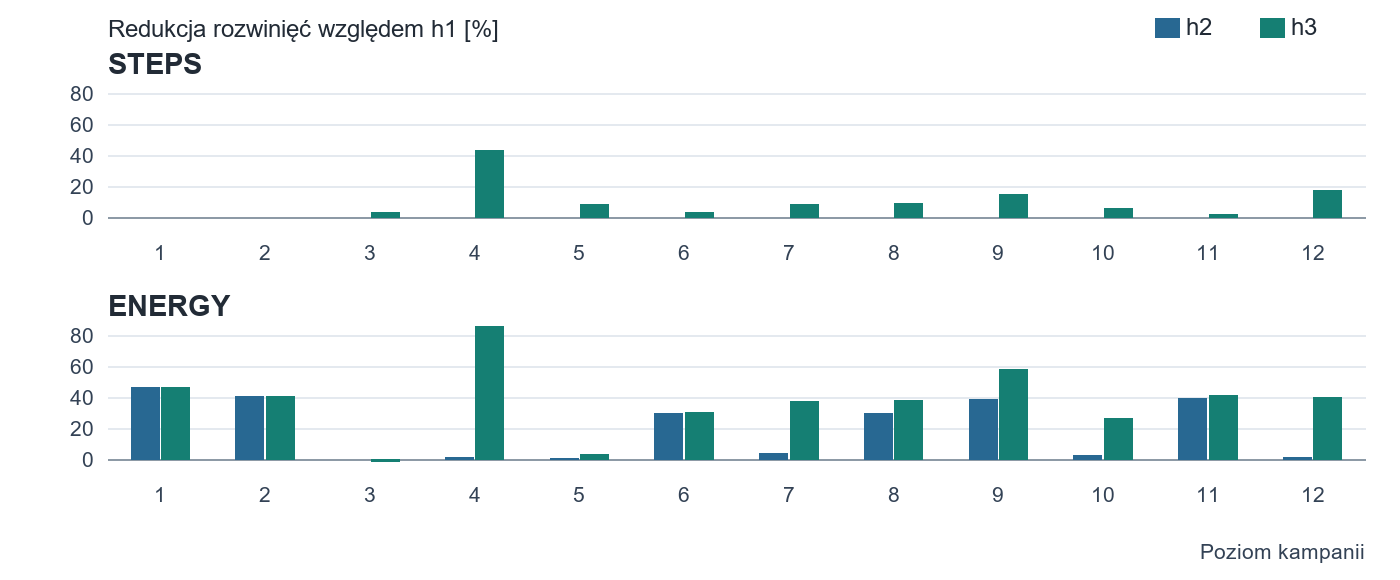
\includegraphics[width=0.91\linewidth]{figures/rozwiniete_stany.png}
\caption{Zmiana liczby rozwinięć względem $h_1$ na poszczególnych planszach. Słupek dodatni oznacza redukcję, a ujemny wzrost liczby rozwinięć.}
\label{fig:expanded}
\end{figure}

Na \emph{Wielkim magazynie} w ENERGY $h_3$ zmniejszyła liczbę rozwinięć z 98\,730 do 59\,039, czyli o 40,2\%. Mediana czasu spadła z 16,86 do 10,07 s. Koszt planu dla wszystkich trzech heurystyk wynosił 7340,57 J. Na pierwszej planszy w STEPS wszystkie warianty rozwinęły po 41 stanów, a $h_3$ potrzebowała 5,49 ms wobec 3,95 ms dla $h_1$. Przy małej przestrzeni stanów przygotowanie grafu może więc zwiększyć czas wyszukiwania.

\begin{table}[H]
\centering\small
\caption{Wyniki dla poziomu 12, \emph{Wielki magazyn}. Wartości dla $h_2$ w ENERGY pochodzą z dwóch udanych prób.}
\label{tab:last-level}
\begin{tabular}{@{}llrrr@{}}
\toprule
Tryb & Heurystyka & Rozwinięcia & Odkryte stany & Mediana [s] \\
\midrule
\LastLevelRows
\bottomrule
\end{tabular}
\end{table}

\subsection{Wpływ funkcji kosztu}
Na dziewięciu poziomach plany wyznaczone z $h_1$ w obu trybach miały tę samą długość i energię. Na trzech poziomach ENERGY zmniejszyło zużycie energii o 0,82--2,07\%. W \emph{Ciężarowcu} i \emph{Wielkim magazynie} wymagało to dodatkowych ruchów. W \emph{Lodowych beczkach} oba plany liczyły po 31 ruchów i 7 pchnięć, lecz miały inny przebieg i koszt energetyczny.

\begin{table}[H]
\centering\small
\caption{Poziomy, na których ENERGY zmniejszyło zużycie energii względem STEPS dla $h_1$.}
\label{tab:criteria}
\begin{tabular}{@{}lrrrrr@{}}
\toprule
Poziom & Ruchy S/E & STEPS [J] & ENERGY [J] & Zysk [J] & Zysk [\%] \\
\midrule
\EnergyTradeoffRows
\bottomrule
\end{tabular}
\end{table}

\begin{figure}[H]
\centering
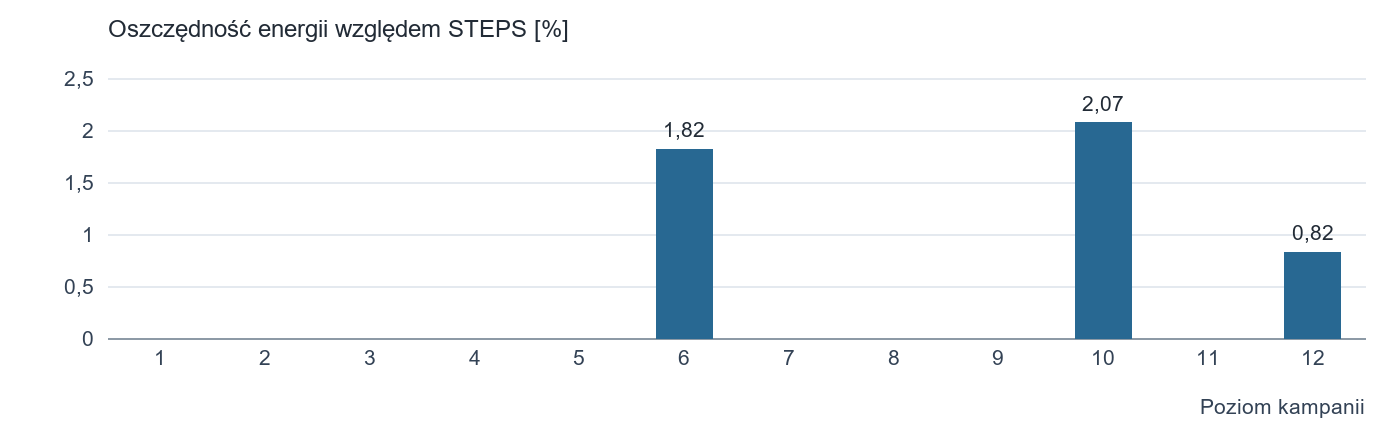
\includegraphics[width=0.91\linewidth]{figures/oszczednosc_energii.png}
\caption{Procentowa oszczędność energii planu ENERGY względem planu STEPS przy heurystyce $h_1$.}
\label{fig:savings}
\end{figure}

\clearpage
\section{Wnioski i ograniczenia}
\begin{enumerate}
\item Wspólny model ruchu zapewnił zgodność planowania i odtwarzania. Wszystkie uzyskane plany doprowadziły do rozwiązania przy deklarowanej energii i długości.
\item $h_3$ dała największą łączną redukcję rozwinięć w obu trybach. W ENERGY $h_2$ poprawiła wynik względem Manhattan już przez uwzględnienie minimalnej pracy potrzebnej do pchania obiektu.
\item Wybór kryterium zmieniał plan. Na dwóch poziomach dodatkowe ruchy pozwoliły uzyskać mniejszy koszt energetyczny, a na jednym poziomie koszt zmalał przy tej samej długości planu.
\end{enumerate}

Zakres pomiarów obejmuje 12 plansz przygotowanych przez zespół, jeden komputer i trzy powtórzenia na konfigurację. Czasy zależą od sprzętu i obciążenia systemu. Model fizyczny jest dyskretny, a detekcja blokad w solverze obejmuje narożniki. Wyszukiwanie na głównym wątku może chwilowo blokować interfejs. Kolejne badania mogą objąć szerszy zestaw plansz, porównanie wariantów detekcji blokad, wpływ zmiany $F_{\max}$ oraz planowanie w osobnym wątku.

\section{Odtwarzalność, kod i podział prac}
Repozytorium zespołu: \url{https://github.com/Man1ek27/Sokoban-ai}. Pomiar wykonano na lokalnym kodzie opartym na commicie \texttt{2fef64ff0088}, z implementacją $h_2$ i $h_3$ dołączoną do projektu. Kolumna \texttt{code\_sha256} w danych surowych identyfikuje dokładny zestaw plików GDScript i JSON użyty podczas pomiaru.

Grę uruchamia się przez otwarcie \texttt{project.godot} w Godot 4.7.2 i naciśnięcie F5. Polecenia testów i benchmarku, wykonywane z katalogu projektu, są podane poniżej. Import jest potrzebny przy pierwszym uruchomieniu od zera.

\begin{samepage}
\begin{quote}\footnotesize\ttfamily
\detokenize{godot --headless --editor --path . --import}\\
\detokenize{godot --headless --path . --script res://tests/physics_test.gd}\\
\detokenize{godot --headless --path . --script res://tests/game_integration_test.gd}\\
\detokenize{godot --headless --path . --script res://sprawozdanie/benchmark.gd}
\end{quote}
\end{samepage}

Testy fizyki i solvera obejmowały 97 sprawdzeń, a test integracji gry 80. Wszystkie przeszły. Dane surowe zawierają 216 wierszy w \path{benchmark_raw.csv}. Agregaty dla 72 konfiguracji są w \path{benchmark_summary.csv}. Wykresy, tabele i agregaty można odtworzyć poleceniem \texttt{python} \path{sprawozdanie/aggregate_benchmark.py} (Python 3, Pillow).

\begin{table}[H]
\centering
\caption{Podział odpowiedzialności w zespole.}
\begin{tabularx}{\linewidth}{@{}p{3.1cm}X@{}}
\toprule
Osoba & Zakres prac \\
\midrule
Radosław Firlej & A*, reprezentacja stanu, trzy heurystyki, wykrywanie blokad narożnych, uruchomienie solvera bez okna i porównanie heurystyk. \\
Alicja Borek & Środowisko Godot, HUD, animacje, integracja AI z rozgrywką, konfiguracja siły i wizualizacja planu. \\
Mariusz Wątroba & Model fizyczny, przygotowanie kampanii poziomów, nowe mechaniki oraz testy fizyczne. \\
\bottomrule
\end{tabularx}
\end{table}

\section*{Źródła}
\begin{enumerate}
\item Materiały do przedmiotu \emph{Sztuczna inteligencja w grach i rozszerzonej rzeczywistości}, 2026.
\item Repozytorium zespołu: \href{https://github.com/Man1ek27/Sokoban-ai}{Sokoban AI (GitHub)}, stan z 12.11.2026.
\item Wyniki benchmarku z 12.11.2026: \path{benchmark_raw.csv} oraz \path{benchmark_summary.csv}.
\end{enumerate}

\end{document}
